% !TeX root = Bericht_main.tex
\newpage
\subsection{Aufgabe 32}
In Aufgabe 32 beschäftigen wir uns nochmal mit dem Grenzfall 
Diffusion $\to 0$. Dabei werden wir nun das Streamline Diffusion Verfahren (SDV) verwenden (vgl. Theorieteil Abschnitt 1.4).

\begin{figure}[H]
	\centering
	\captionabove{Vergleich unterschiedlicher Verfahren bei Diffusion 0.00001 zum Zeitpunkt $t=1$}
	\subfigure[FEM lv2]{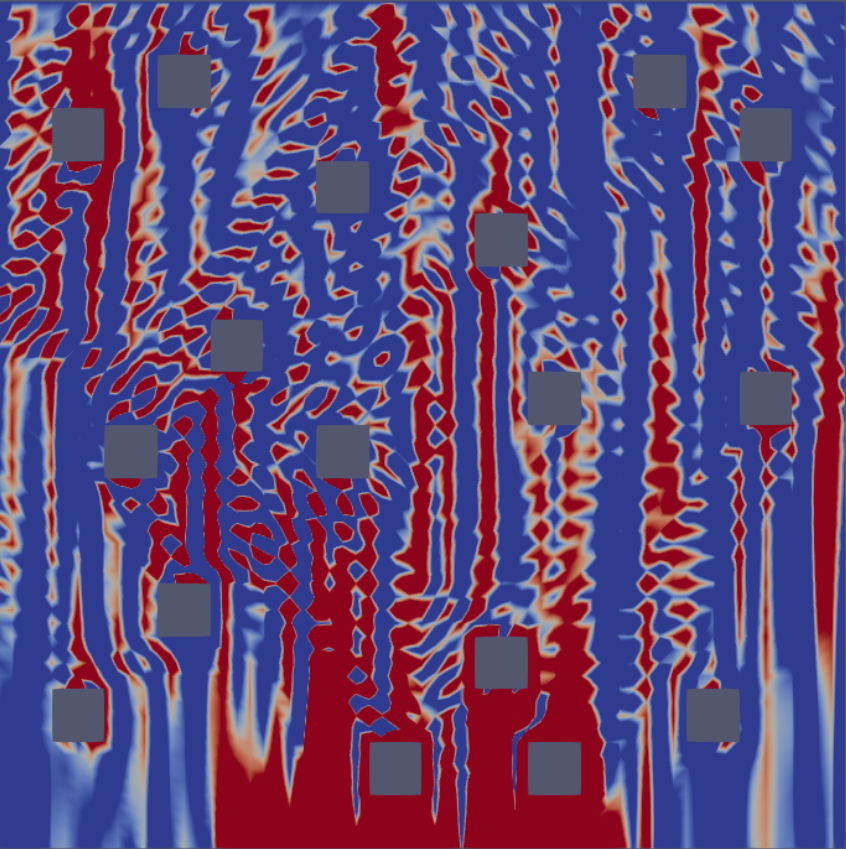
\includegraphics[width=0.32\textwidth]{../Aufgabe27/b/reaction=5_diffusion=1e-05/animation40.png}}	 
	\subfigure[Serendipity lv2]{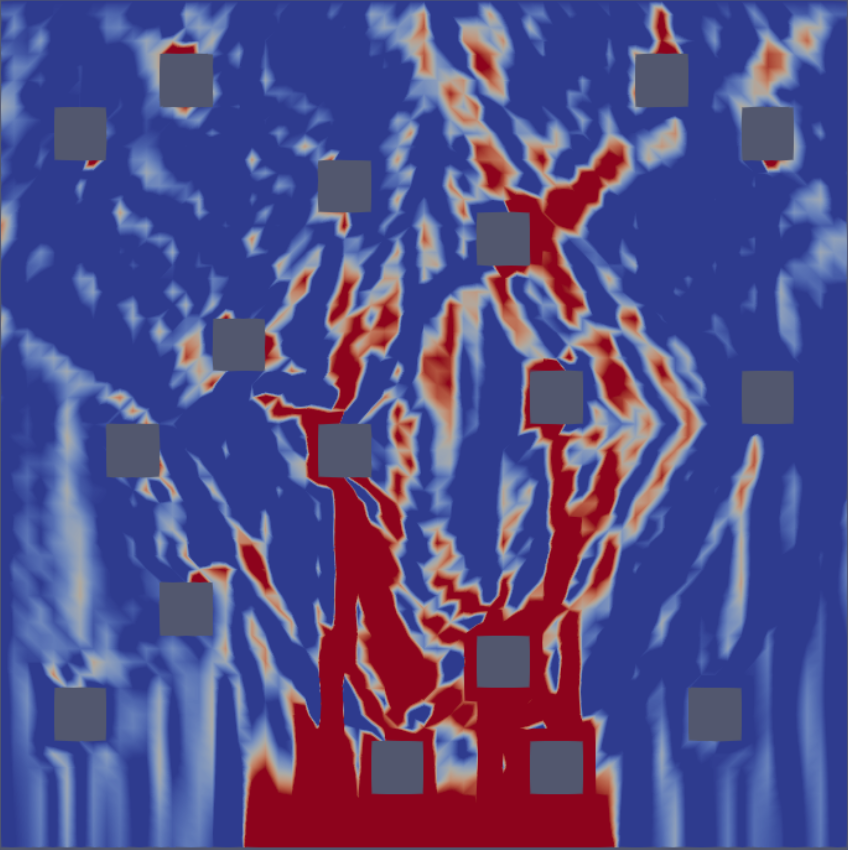
\includegraphics[width=0.32\textwidth]{../Aufgabe27/c/serendipity_lvl=2_reaction=5_diffusion=1e-05/animation40.png}}
    \subfigure[Serendipity lv3] {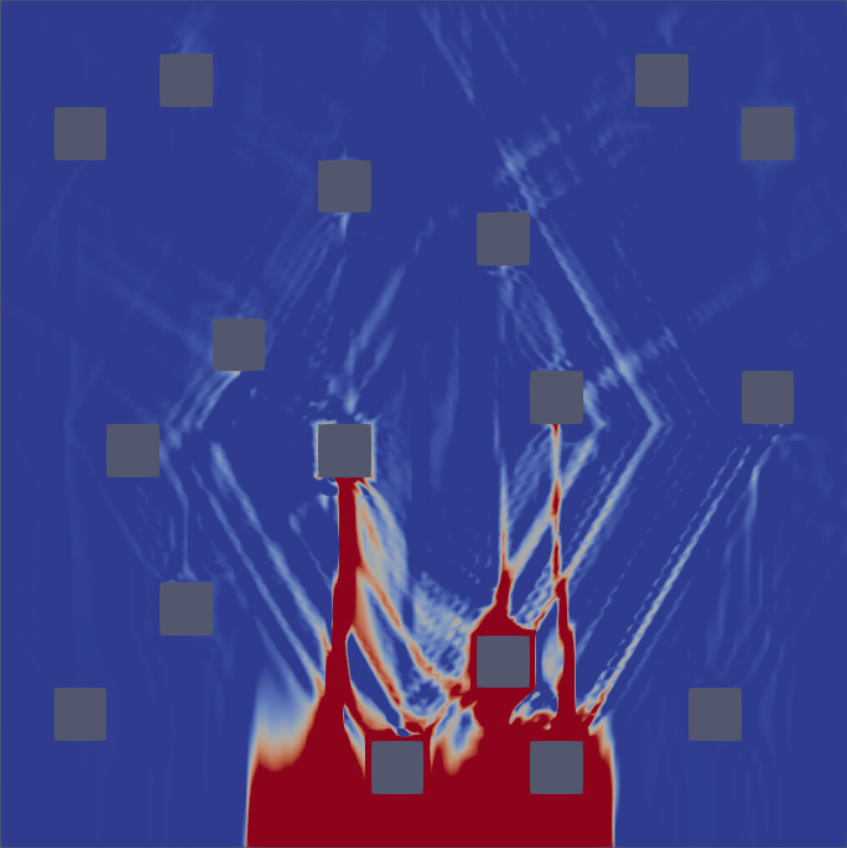
\includegraphics[width=0.32\textwidth]{../Aufgabe27/c/serendipity_lvl=3_reaction=5_diffusion=1e-05/animation40.png}}
    \subfigure[SDV Delta 0.025]{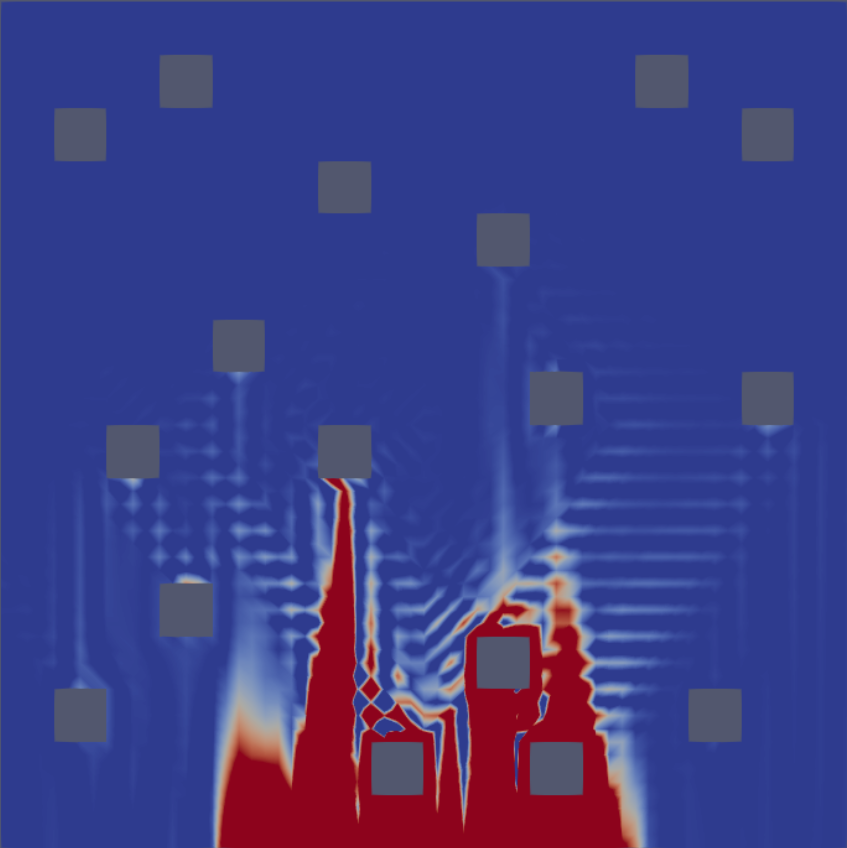
\includegraphics[width=0.32\textwidth]{../Aufgabe32/delta=0.025_diffusion=1e-05/animation40.png}}
    \subfigure[SDV Delta 0.1]{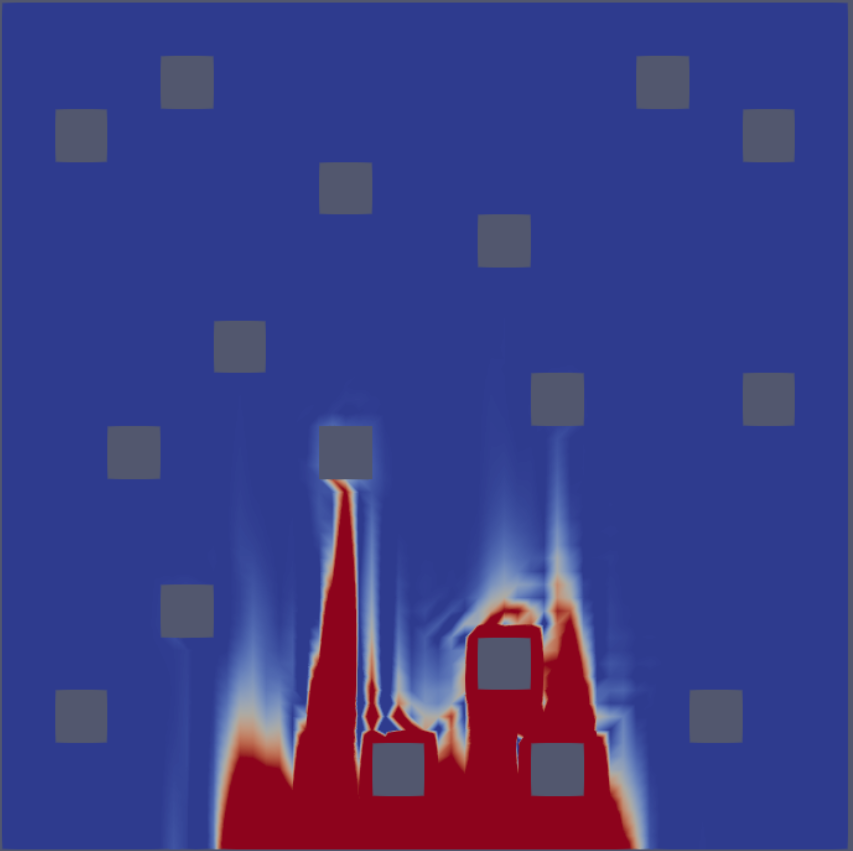
\includegraphics[width=0.32\textwidth]{../Aufgabe32/delta=0.1_diffusion=1e-05/animation40.png}}  
    \subfigure[SDV Delta 5]{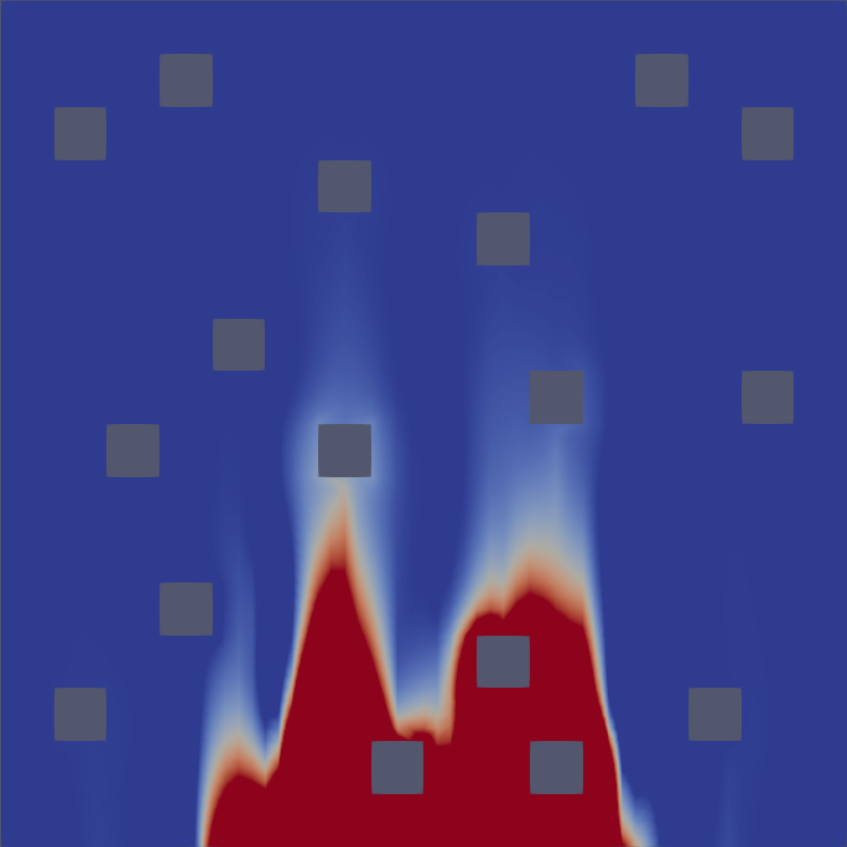
\includegraphics[width=0.32\textwidth]{../Aufgabe32/delta=5_diffusion=1e-05/animation40.png}}
\end{figure}

Wie wir anhand der Bilder zum Zeitpunkt $t=1$ erkennen können, eignen sich unsere bisherigen Verfahren (FEM und Serendipity) nicht für die sehr geringe Diffusion 0.000001. Im Gegensatz dazu steht das Streamline Diffusion Verfahren. Dabei erzeugen wir mithilfe von $\delta_K$ eine 'künstliche' Diffusion. Schon bei einem $\delta_K$ in der Größenordnung unserer Gitterweite ($\approx 0.025$)
erhalten wir eine deutlich bessere Lösung, als zuvor noch mit den bisherigen Verfahren. Bei einem sehr großen Delta 
($\approx 5$) sieht unsere Lösung glatt aus. Dies ist der Tatsache geschuldet, dass wir durch das große Delta auch eine große 'künstliche' Diffusion erzeugt haben. Noch deutlicher sieht man das bei noch geringeren Diffusionen:

\begin{figure}[H]
	\centering
	\captionabove{Vergleich unterschiedlicher Verfahren bei Diffusion 0.000001 zum Zeitpunkt $t=1$}
	\subfigure[FEM lv2]{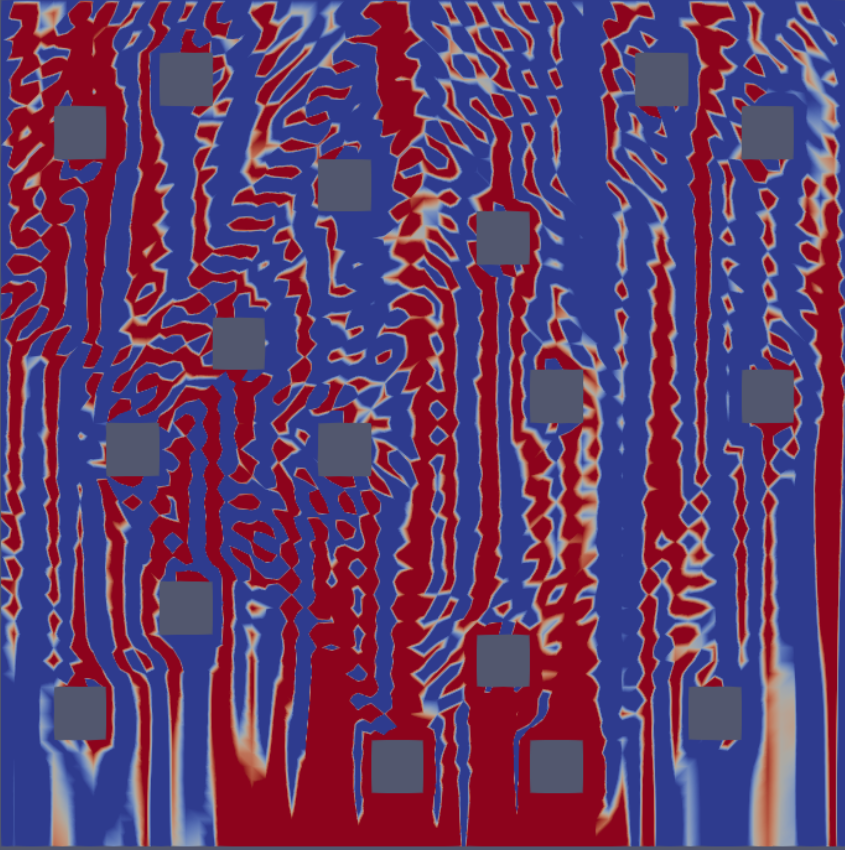
\includegraphics[width=0.32\textwidth]{../Aufgabe27/b/reaction=5_diffusion=1e-06/animation40.png}}	 
	\subfigure[Serendipity lv2]{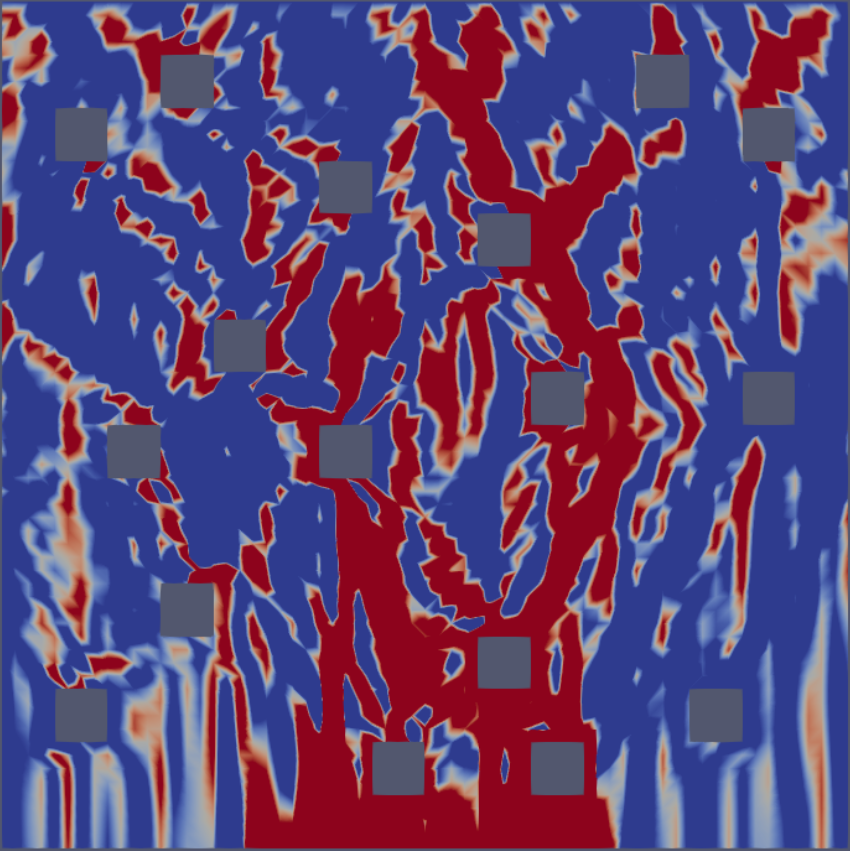
\includegraphics[width=0.32\textwidth]{../Aufgabe27/c/serendipity_lvl=2_reaction=5_diffusion=1e-06/animation40.png}}
	\subfigure[Serendipity lv3] {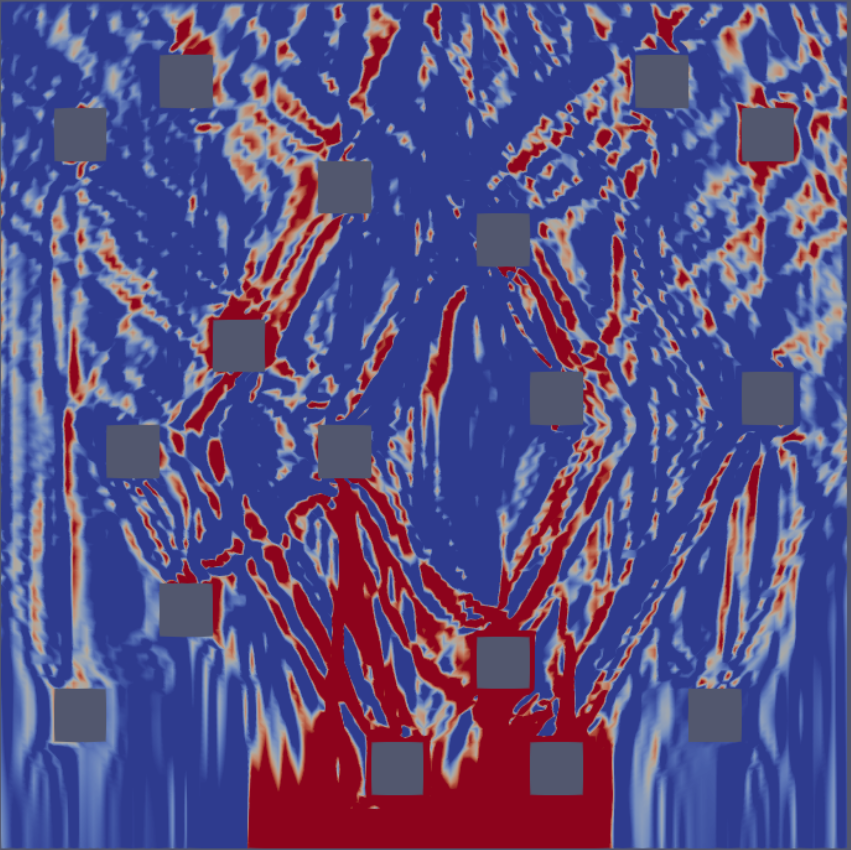
\includegraphics[width=0.32\textwidth]{../Aufgabe27/c/serendipity_lvl=3_reaction=5_diffusion=1e-06/animation40.png}}
	\subfigure[SDV Delta 0.025]{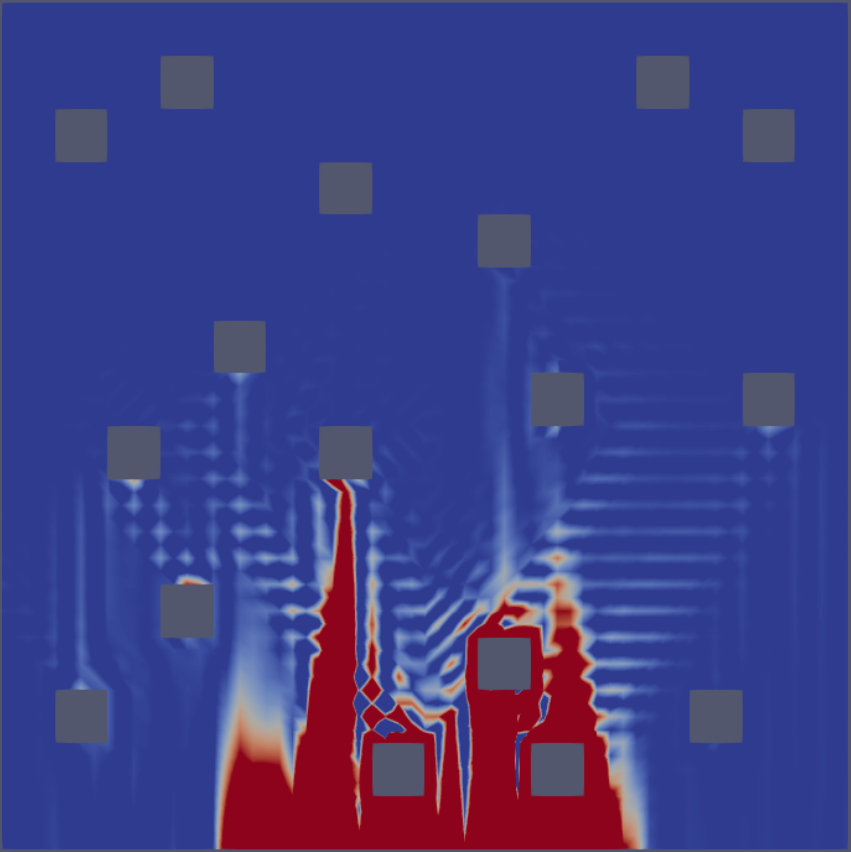
\includegraphics[width=0.32\textwidth]{../Aufgabe32/delta=0.025_diffusion=1e-06/animation40.png}}
	\subfigure[SDV Delta 0.1]{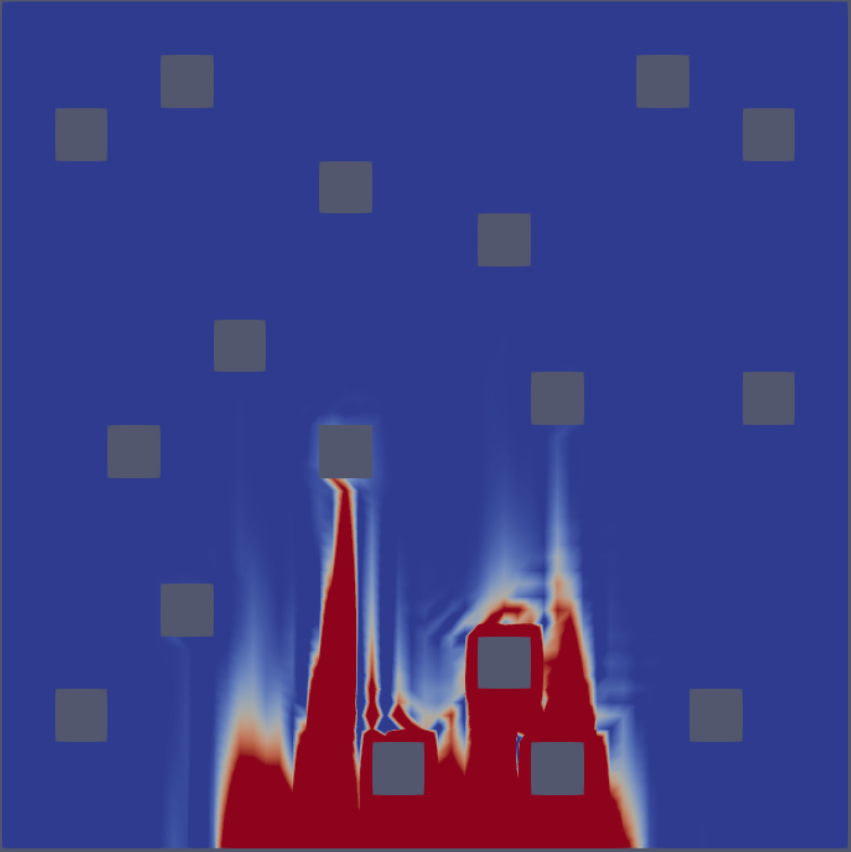
\includegraphics[width=0.32\textwidth]{../Aufgabe32/delta=0.1_diffusion=1e-06/animation40.png}}  
	\subfigure[SDV Delta 5]{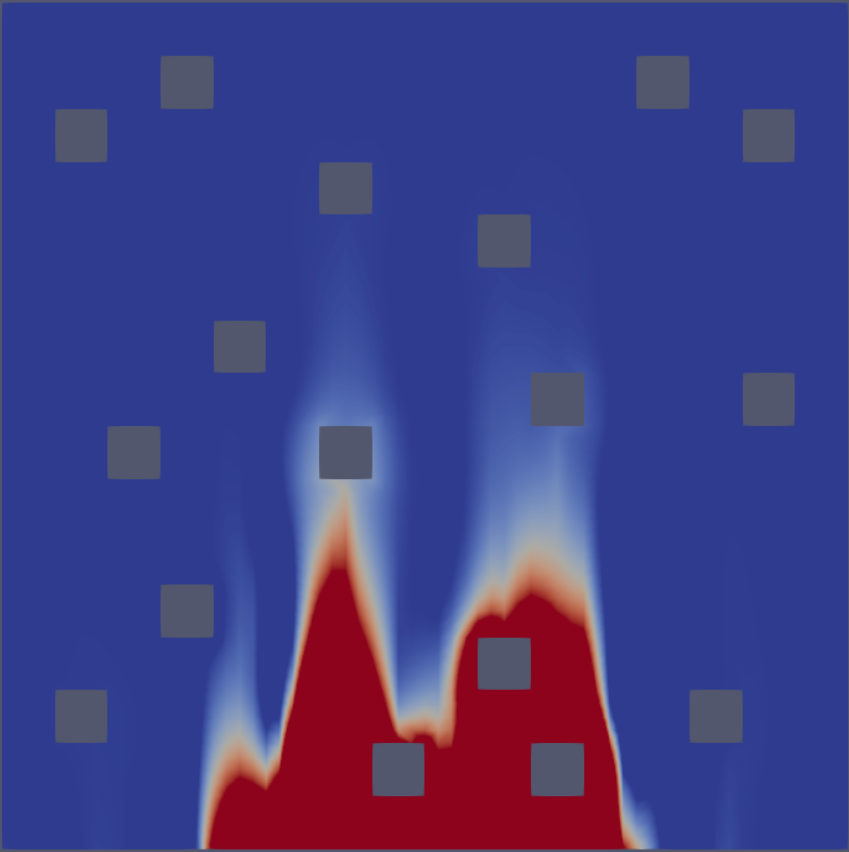
\includegraphics[width=0.32\textwidth]{../Aufgabe32/delta=5_diffusion=1e-06/animation40.png}}
\end{figure}

Insgesamt haben wir damit durch die unstetige Wahl der Testfunktionen im SDV ein bereits brauchbares Verfahren für das Problem Diffusion $\to 0$ gefunden, bei dem die bisherigen Verfahren  starke Oszillationen aufwiesen. 
